%%%%%%%%%%%%%%%%%%%%%%%%%%%%%%%%%%%%%%%%%%%%%%%%%%%%%%%
\documentclass{article}
\usepackage[utf8]{vietnam}
\usepackage{amsmath}
\usepackage{graphicx}
\usepackage{float} 
\begin{document}
%%%%%%%%%%%%%%%%%%%%%%%%%%%%%%%%%%%%%%%%%%%%%%%%%%%%%%%
\section{Tổng quan về mật mã khóa công khai}
\subsection{Lịch sử}
Ý tưởng về hệ thống mã hóa khóa công khai được Martin Hellman, Ralph Merkle và Whitfield Diffie tại Đại học Stanford giới thiệu vào năm 1976.


Sách:

Diffie, W.; Hellman, M.E. (November 1976). "New directions in cryptography". IEEE Transactions on Information Theory





\subsection{Khái niệm:}


Mật mã khóa công khai (public-key) là hệ mã không đối xứng, nghĩa là sử dụng hai khóa liên đới cho việc mã hoá và giải mã thay vì một khóa duy nhất như trong các hệ mã cổ điển (hay còn gọi là hệ mã đối xứng). Việc này đáp ứng được các yêu cầu trong các ứng dụng về bảo mật riêng tư, phân phối khóa, và xác thực điện tử.

Lưu ý:

Một hệ mật khóa công khai không bao giờ cung cấp độ mật vô điều kiện - thực tế, đó là hàm cửa sập một chiều (a trapdoor one-way function).

\subsection{Mô hình hệ mật khóa công khai tổng quát}

\begin{figure}[H]
    \centering
    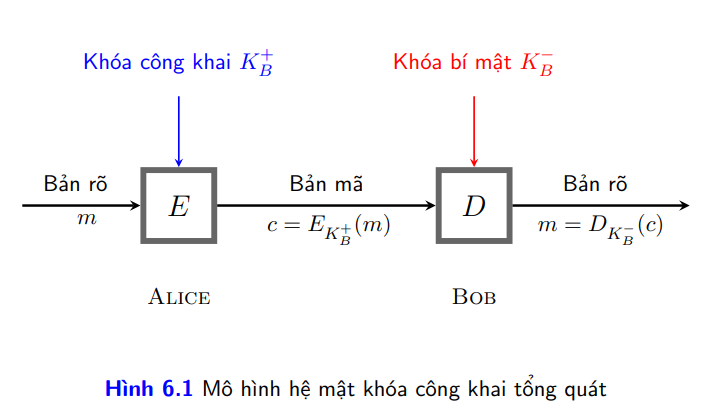
\includegraphics[scale = 0.5]{pictures/public.png}
    \caption{Mô hình hệ mật khóa công khai tổng quát}
\end{figure}


Ý tưởng:
\begin{itemize}
    \item Mỗi người dùng: sử dụng một cặp khóa (khóa công khai, khóa bí mật)
          \begin{itemize}
              \item  Khóa công cộng (public key): được công bố rộng rãi và được sử dụng trong mã hóa thông tin
              \item  Khóa riêng (private key): chỉ do một người nắm giữ và được sử dụng để giải mã thông tin đã được mã hóa bằng khóa công cộng tương ứng
          \end{itemize}

    \item Mã hóa: A muốn gửi thông điệp cho B - mã hóa bằng khóa công khai của B
          $$y = E(e_B, x)$$

    \item Giải mã: B giải mã bằng khóa bí mật của mình
          $$x = D(d_B, y)$$

    \item Hàm mã hóa và giải mã có thể đổi chỗ
\end{itemize}

Trong đó:
\begin{itemize}
    \item  Các phương pháp mã hóa này khai thác những ánh xạ f mà
          \begin{itemize}
              \item  Biết x, tính y=f(x) dễ dàng
              \item   Biết y, việc thực hiện ánh xạ ngược f –1 tính x là rất khó
          \end{itemize}
          Hàm f có tính chất trên thường gọi là hàm một chiều
    \item   Ví dụ: Cho các số nguyên tố p1, p2, ... , pn
          \begin{itemize}
              \item   Tính N= p1* p2* ... * pn- dễ
              \item    Ngược lại, biết N, tìm p1, p2, ... , pn là khó
          \end{itemize}
\end{itemize}


Hàm cửa sập (trap door):
\begin{itemize}
    \item  Để xây dựng hệ mã khóa công khai - thường dùng hàm một chiều đặc biệt có tham số/cửa sập
          \begin{itemize}
              \item  Hàm mã hóa - là hàm cửa sập
              \item  Khóa (bí mật) - chính là thông tin tham số - bẫy trap door
          \end{itemize}
\end{itemize}


\subsection{Những hệ mật khóa công khai quan trọng nhất}
\begin{itemize}
    \item  RSA: dựa trên độ khó của phép phân tích các số nguyên lớn.
    \item   Merkle-Hellman Knapsack: và các hệ liên quan dựa trên độ khó của bài toán subset sum (được biết là NP-complete). Tuy nhiên, có nhiều hệ mật dựa trên bài toán sắp ba lô đã được chứng minh là không bảo mật.
    \item    McEliece: dựa trên bài toán giải mã của một mã tuyến tính (cũng được cho là NP-complete).
    \item     ElGamal: dựa trên bài toán Logarit rời rạc trên trường hữu hạn.
    \item      Chor-Rivest: là một hệ sắp ba lô nhưng được xem là bảo mật.
    \item       Elliptic Curve: là sự cải tiến của các hệ mật khác, chẳng hạn tương tự ElGamal nhưng dựa trên các đường cong elíp thay vì trường hữu hạn. Ưu điểm của các hệ mật dạng này là có thể duy trì được độ bảo mật với khóa nhỏ hơn thông thường.
\end{itemize}

\section{Hệ mật RSA}
\subsection{Lịch sử}
Hệ mật RSA, được phát triển bởi Ron Rivest, Adi Shamir và Leonard Adleman (1977), có thể được sử dụng trong bảo mật dữ liệu và công nghệ chữ ký điện tử.
\subsection{Ý tưởng}
Bảo mật của RSA dựa trên giả thuyết không có các thuật toán đủ nhanh để khai triển luỹ thừa một số. Qui trình áp dụng RSA gồm hai bước:
\begin{enumerate}
    \item  Lựa chọn (sinh) cặp khóa công khai và khóa bí mật
    \item   Thực hiện thuật toán mã hoá và thuật toán giải mã
\end{enumerate}



\subsection{Mô tả hệ mật}

\begin{itemize}
    \item Các phép tính được thực hiện trên $Z_n$ với $n = p \cdot q$.
    \item $S = \langle P, C, K, E, D \rangle$
    \begin{itemize}
        \item $n = pq$ với $p$ và $q$ là hai số nguyên tố lẻ phân biệt. $\phi(n) = (p-1)(q-1)$
        \item $P = C = Z_n$
        \item $K = \{ (n, p, q, a, b) : n = pq, p, q$ là số nguyên tố, $ab \equiv 1 \mod \phi(n) \}$
    \end{itemize}
\end{itemize}

Với mỗi $k = (n, p, q, a, b) \in K$, định nghĩa:
\begin{align*}
    e_k(x) &= x^b \mod n \\
    d_k(y) &= y^a \mod n
\end{align*}
với $x, y \in Z_n$.




\subsection{Sinh cặp khóa công khai - bí mật}

\begin{enumerate}
    \item   Chọn hai số nguyên tố đủ lớn, $p$ và $q$ 
    \item    Tính toán $n = pq$ và $\phi(n) = (p - 1)(q - 1)$ 
    \item     Chọn một số, $e$ $(1 < e < \phi(n))$ sao cho $\text{gcd}(e, \phi(n)) = 1$. Giá trị $e$ sẽ được sử dụng trong mã hoá
    \item     Tìm một số $d$ sao cho $ed - 1$ chia hết cho $\phi(n)$, hay nói cách khác $d = e^{-1} \mod \phi(n)$. Giá trị $d$ sẽ được sử dụng để giải mã 
    \item     Công khai khóa $K^+_B$  = (n, e)  và giữ bí mật khóa $K^-_B$  = (n, d) 
\end{enumerate}



\begin{figure}[H]
    \centering
    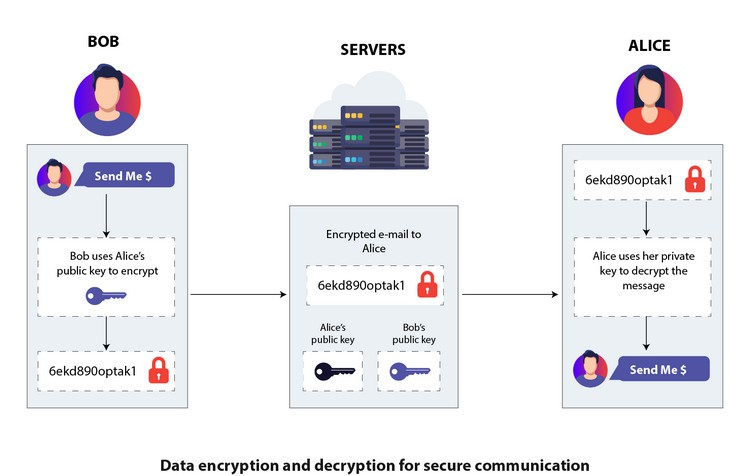
\includegraphics[scale = 0.4]{pictures/Bob_Alice.jpg}
    \caption{Thuật toán mã hoá (Alice) và thuật toán giải mã (Bob)}
\end{figure}


Mã hoá (Alice):

 

Giả sử Alice muốn gửi cho Bob một mẫu bit, hoặc một số $m$ sao cho $m < n$. Để mã hoá, Alice thực hiện tính luỹ thừa, $m^e$, sau đó tính toán số dư khi đem chia $m^e$ cho $n$. Vì vậy, giá trị được mã hoá ($c$) của bản tin $m$ là:  $c = m^e \mod n $


Giải mã (Bob):

Để giải mã đoạn tin mã hoá nhận được ($c$), Bob tính toán: $ m = c^d \mod n $. Việc này đòi hỏi phải sử dụng khóa bí mật $(n, d)$.



Ví dụ:

Giả sử B chọn $p = 101$ và $q = 113$, khi đó $n = 11413$ và $\phi(n) = 11200$.

Giả sử B chọn $b = 3533$, khi đó bằng thuật toán Euclidean mở rộng ta tính được
\[a = b^{-1} \equiv 6597 \pmod{11200}.\]

B công khai bộ $(n = 11413, b = 3533)$.



Bây giờ giả sử A muốn gửi từ hiện $9726$ cho B, A sẽ tính 
\[9726^{3533} \equiv 5761 \pmod{11413},\] 
là từ mã. 

Khi B nhận được $5761$, B sẽ tính 
\[5761^{6597} \equiv 9726 \pmod{11413},\] 
và thu được từ hiện A muốn gửi.





\subsection{Áp dụng hệ mật RSA}

\begin{enumerate}
    \item Sinh hai số nguyên tố có giá trị lớn: $p$ và $q$
    \item Tính $n = pq$ và $\phi(n) = (p - 1)(q - 1)$
    \item Chọn ngẫu nhiên một số nguyên $e$ $(1 < e < \phi(n))$ thỏa $\text{gcd}(e, \phi(n)) = 1$
    \item Tính giá trị $d = e^{-1} \mod \phi(n)$ (bằng thuật toán Euclide mở rộng)
    \item Công bố giá trị $(n, e)$ (khóa công khai)
    \item Giữ bí mật giá trị $(p, q, d)$ (khóa bí mật)
\end{enumerate}


 




%%%%%%%%%%%%%%%%%%%%%%%%%%%%%%%%%%%%%%%%%%%%%%%%%%%%%%%
\section*{References:}
Diffie, W.; Hellman, M.E. (November 1976). "New directions in cryptography". IEEE Transactions on Information Theory


https://ieeexplore.ieee.org/document/1055638





Slide mật mã thầy Hân

Slide mật mã thầy Nam


\end{document}
%%%%%%%%%%%%%%%%%%%%%%%%%%%%%%%%%%%%%%%%%%%%%%%%%%%%%%%

